\normaltrue
\correctionfalse

%\UPSTIidClasse{11} % 11 sup, 12 spé
%\newcommand{\UPSTIidClasse}{12}

\exer{Mouvement RTR  $\star$ \label{CIN:02:B2:13:1025}}
\setcounter{question}{0}\marginnote{\xpComp{CIN}{02}}%\xpComp{CIN}{02}%\UPSTIcompetence[2]{C2-05}
%\UPSTIcompetence[2]{B2-13}}
\index{Compétence C2-05}
\index{Compétence B2-13}\index{Compétence CIN-02}

\ifcorrection
\else
\marginnote{\textbf{Pas de corrigé pour cet exercice.}}
\fi

\ifprof
\else
Soit le mécanisme suivant. On a $\vect{AB}=R\vect{i_1}$ et $\vect{BC}=\lambda(t)\vect{i_2}+r\vj{2}$.
\begin{figure}[H]
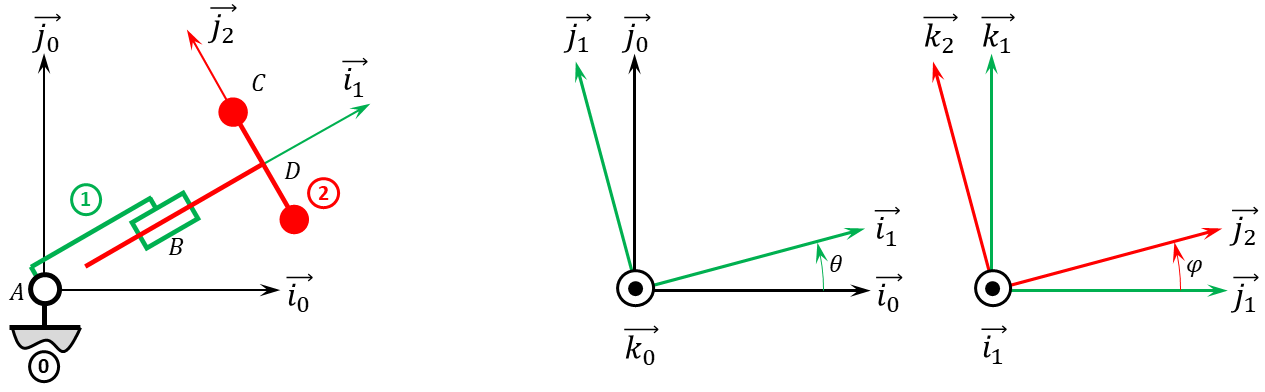
\includegraphics[width=\linewidth]{1025_01}
\end{figure}
\fi

\question{Déterminer $\vectv{B}{2}{0}$, $\vectv{D}{2}{0}$, $\vectv{C}{2}{0}$}.
\ifprof~\\
\else
\fi

\question{Déterminer $\vectg{B}{2}{0}$, $\vectg{D}{2}{0}$, $\vectg{C}{2}{0}$}.
\ifprof~\\
\else
\fi



\ifprof
\else
\marginnote{Corrigé  voir \ref{CIN:02:B2:13:1025}.}
\fi